\documentclass[text07.tex]{subfiles}
\begin{document}
%
% section 6.2
%
\section{インターネットのキホン}
\refstepcounter{PagePtr}\label{P:internet}
\begin{wrapfigure}{r}[10pt]{0.4\textwidth}
	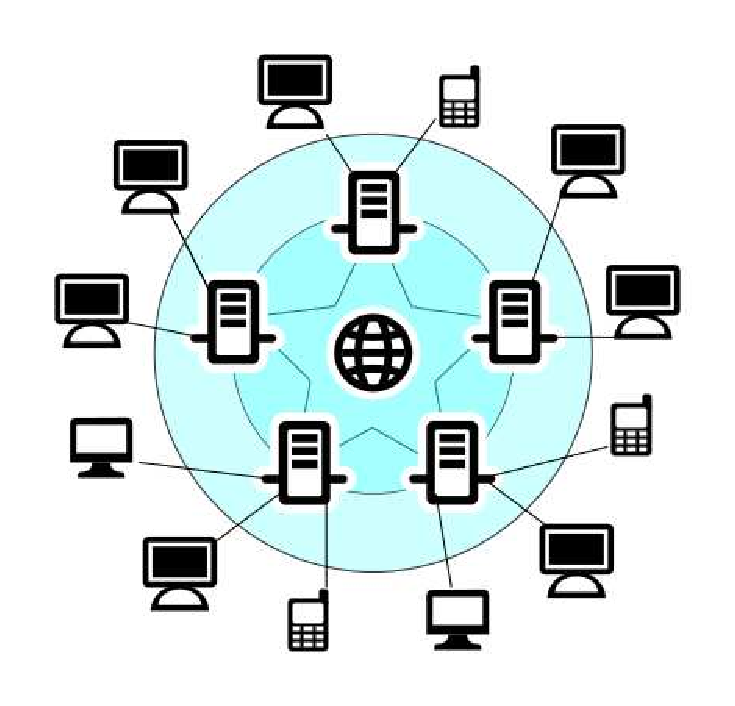
\includegraphics[width=0.4\textwidth]{../../asset/image/ome7-img002.eps}
\end{wrapfigure}

みんなが使っているパソコンやスマートフォンなどをたくさんつなぎ、おたがいに情報の\ruby{交換}{こうかん}ができるようにしたものを「ネットワーク」とよんでいます。
インターネットとは、そのネットワークが数えきれないほどのケーブルなどでおたがいにつながりあい、\ruby{網}{あみ}の目のように世界中に広がっているそのもののことです。

みなさんはすでにインターネットを\ruby{触}{さわ}っています。\\
第一回の\ruby{講義}{こうぎ}でみなさんはwebから画像を自分のラズベリーパイ（PC）に保存しましたね。
あれもインターネットを触ったということになるのです。
網目のように世界中に広がっているネットワークから好きな画像を調べるということは自分のラズベリーパイでインターネットをしたということになります。

さらに、有名な動画サイト“YouTube”のコンピュータもインターネットにつながっています。
そのおかげでインターネットにつながっているパソコンやスマートフォンであればYouTubeの動画を見ることができます。
もちろん、インターネットにつながっていなければYouTubeの動画や画像\ruby{検索}{けんさく}など行うことはできません。
試しにインターネットを\ruby{切断}{せつだん}してみても面白いかもしれません。

\begin{tcolorbox}[title=\useOmetoi,breakable]
  \begin{enumerate}
    \addquiz{みんなが使っているパソコンやスマートフォンなどをたくさんつなぎ、おたがいに情報の交換ができるようにしたものを何というでしょうか。}
  \end{enumerate}
\end{tcolorbox}

\clearpage

%
% subsection 6.2.1
%
\subsection{IPアドレスとは何だろう？}
% \refstepcounter{PagePtr}\label{P:IP}

ネットワークでコンピュータ同士がつながっているときにどうやって通信相手のコンピュータの場所を\ruby{探}{さが}すのでしょうか？

わたしたちの住んでいる場所をしめす住所（英語でアドレス)と同じ考え方を使います。
インターネットの住所のことをIP(アイピー)アドレスと言います。
わたしたち日本人は住所を東京都港区高輪２−３−２３（東海大学高輪キャンパスの住所)のように表します。
コンピュータの場合は\textbf{数字}で表します。
IPアドレスの場合はxxx.xxx.xxx.xxxのように四つの数字を使って表します。
3ケタずつ「\textbf{.}」点（ドット）で区切ります。
xxxは0～255の数字が入ります。

\begin{center}
	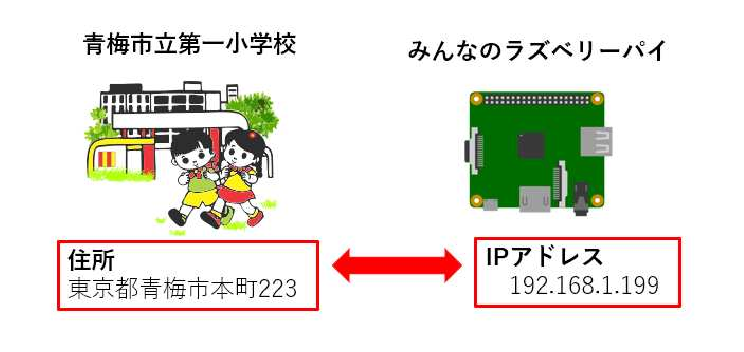
\includegraphics[width=0.8\textwidth]{../../asset/image/ome7-img003}
	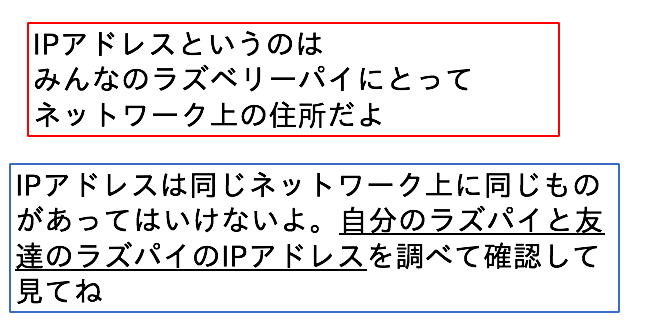
\includegraphics[width=0.8\textwidth]{../../asset/image/ome7-img004.png}
\end{center}

IPアドレスはラズベリーパイのネットワーク上の住所に当たるものです。
一つのネットワークではIPアドレスは同じものがあってはいけません。
例えば、配達する人は同じ住所が世界中にあればどこへ配達したらよいかわからなくなってしまいます。
インターネットの場合も同じです。なのでIPアドレスは同じではいけません。
ですが、例外として他のローカルIPアドレスでは同じになってしまうことはあります。%\textbf{例題７−１で自分のラズベリーパイのIPアドレスを調べましょう}

\clearpage

%
% subsection 6.2.2
%
\subsection{グローバルIPアドレスとローカルIPアドレス}\label{P:slide_p12}
IPアドレスはグローバルIPアドレスとローカル（プライベート）IPアドレスという二つに分けられます。

\begin{center}
	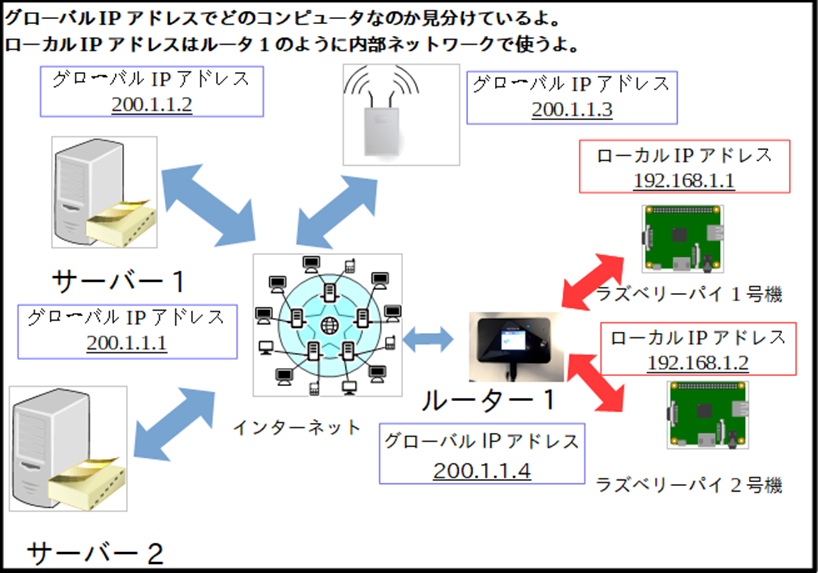
\includegraphics[width=15.0cm]{../../asset/image/ome7-img005.png}
	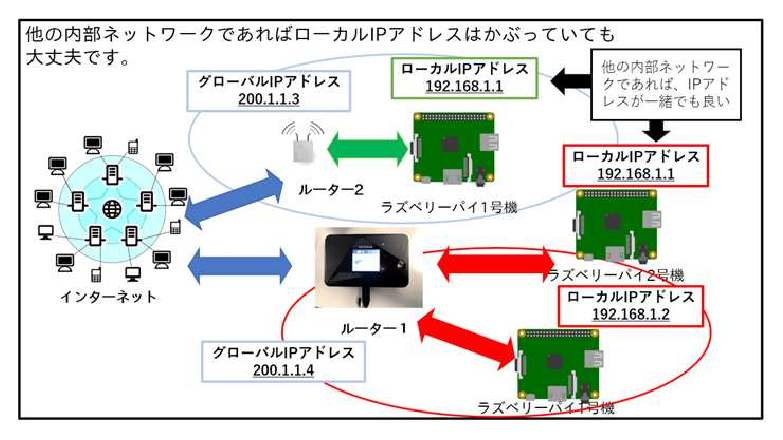
\includegraphics[width=15.0cm]{../../asset/image/ome7-img006}
\end{center}

\begin{tcolorbox}[title=\useOmetoi,breakable]
  \begin{enumerate}
    \addquiz{ローカルIPアドレスがかぶっても良いときはどんなときですか。}
  \end{enumerate}
\end{tcolorbox}



\clearpage

%
% subsection 6.2.3
%
\subsection{IPアドレスを調べてみよう\label{E:checkIP}}

ターミナルにコマンド”hostname
-\texttt{I}”を入力し、自分のラズベリーパイのローカルIPアドレスを確認しよう

\bigskip

{\bfseries 方法}

\begin{center}
	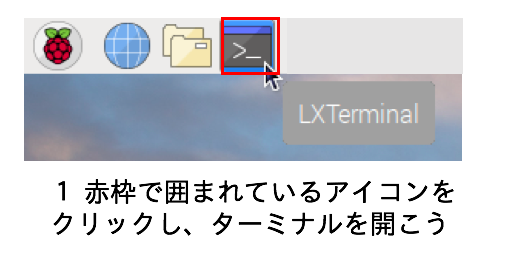
\includegraphics[width=0.85\textwidth]{../../asset/image/ome7-img007.png}
	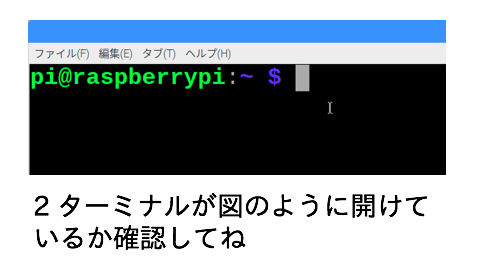
\includegraphics[width=0.85\textwidth]{../../asset/image/ome7-img008.png}
\end{center}

\clearpage

\begin{center}
	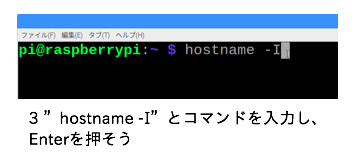
\includegraphics[width=0.85\textwidth]{../../asset/image/ome7-img010.png}
	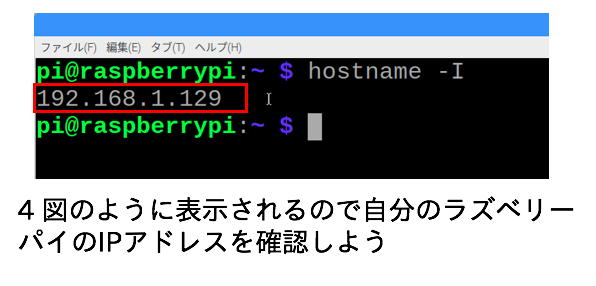
\includegraphics[width=0.85\textwidth]{../../asset/image/ome7-img009.png}
\end{center}


調べた自分のラズベリーパイのIPアドレスを書こう
\begin{center}
	\fbox{
		\parbox{0.8\textwidth}{
		\hspace{0pt}
		\vspace{3\baselineskip}
		}
	}
\end{center}

グループの友達のIPアドレスも教えてもらって書こう
\begin{center}
	\fbox{
		\parbox{0.8\textwidth}{
		\hspace{0pt}
		\vspace{3\baselineskip}
		}
	}
\end{center}

\clearpage

%
% subsection 6.2.4
%
\subsection{インターネットのつながりについて知ろう}\label{P:slide_p14}

教室内では無線通信を利用してインターネットを使用しています。第１回目の授業の最初に\ruby{皆}{みな}さんはインターネット\ruby{接続}{せつぞく}をしました。\ruby{実際}{じっさい}にはどこにつながっているかというと下の図のルータです。

\begin{center}
	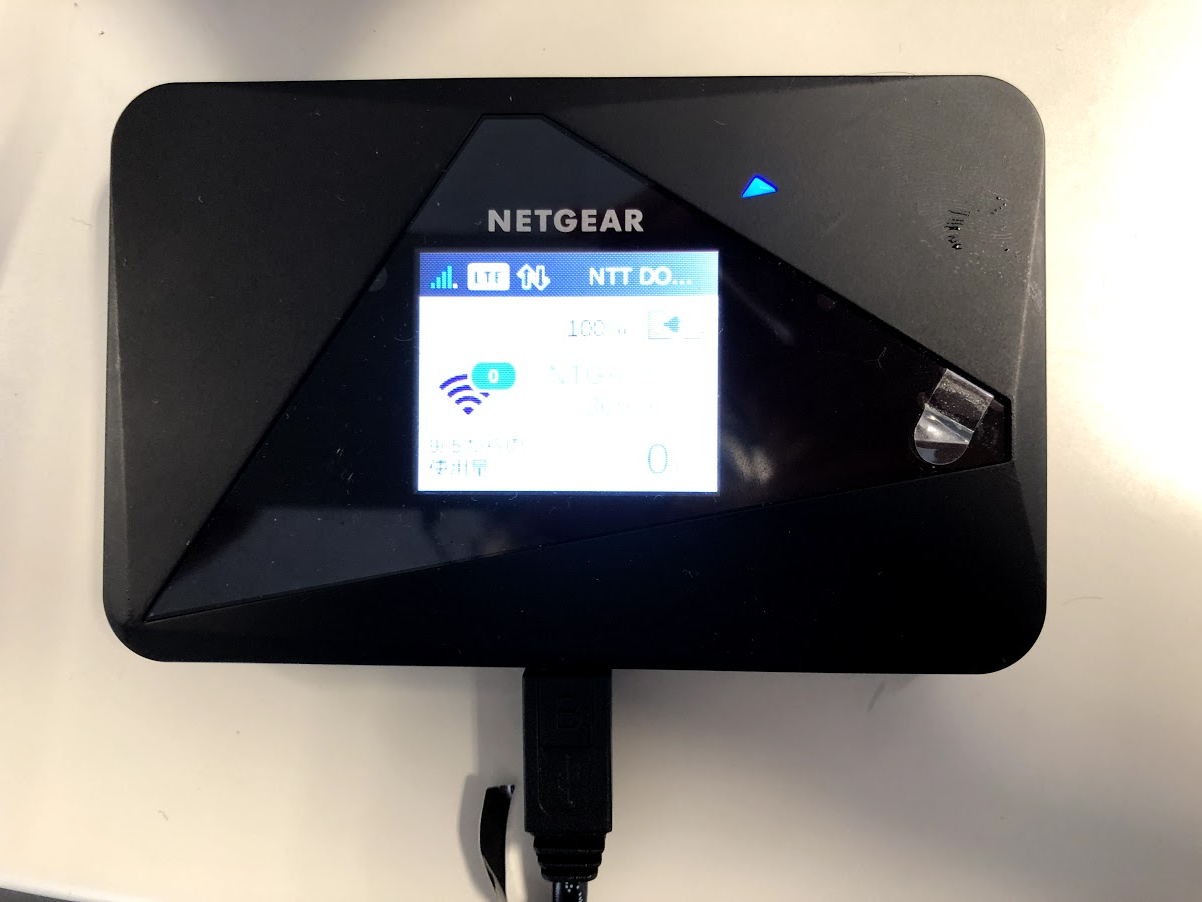
\includegraphics[width=8.186cm]{../../asset/image/ome7-img011.png}
\end{center}

この機械のおかげで、みんなは教室内でインターネットをすることができています。
どういう原理で、みんなのラズベリーパイでインターネットを使用できているか説明していきます。
みんなのラズベリーパイは直接インターネットにつながってはいません。一度、ルータを経由しています。このルータのおかげで\ruby{複数}{ふくすう}のラズベリーパイやPCを同時にインターネットにアクセスさせることができます。以下の図がイメージ図です。

\begin{center}
	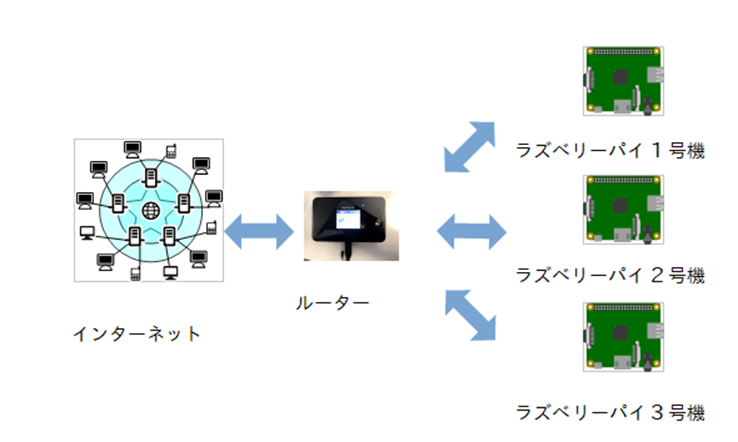
\includegraphics[width=0.85\textwidth]{../../asset/image/ome7-img012.png}
\end{center}

ではどのようにして複数台のラズベリーパイをインターネットに接続しているのでしょうか。それはルータに\textbf{グローバルIPアドレス}というものを\ruby{割}{わ}り当てて、ルータが他のラズベリーパイの代表として通信を行っています。どういうことかわかりづらいので、図でみていきましょう。

\begin{center}
	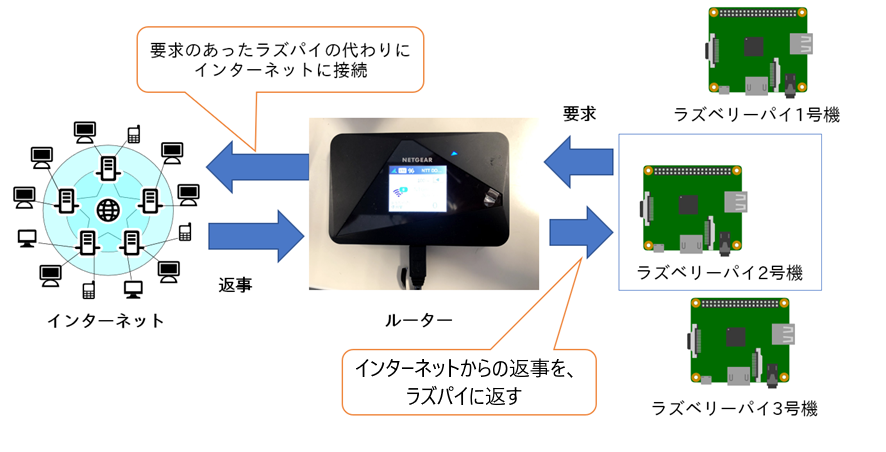
\includegraphics[width=0.85\textwidth]{../../asset/image/ome7-img013.png}
\end{center}


図ではラズベリーパイ2号機がインターネットにアクセスし、何かしらのwebサイトを観たいと要求したとします。その要求はまずルータのところにいき、ラズベリーパイ２号機の代わりにインターネットに接続します。その接続で、ルータはインターネット先から返事をもらい、そのインターネットからの返事をラズベリーパイに返しています。

\begin{center}
	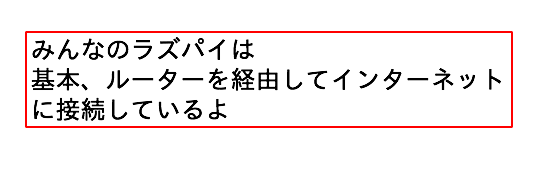
\includegraphics[width=0.85\textwidth]{../../asset/image/ome7-img014.png}
\end{center}

\clearpage

これだけではうまくいかないことがあります。下の図をみてください。

\begin{center}
	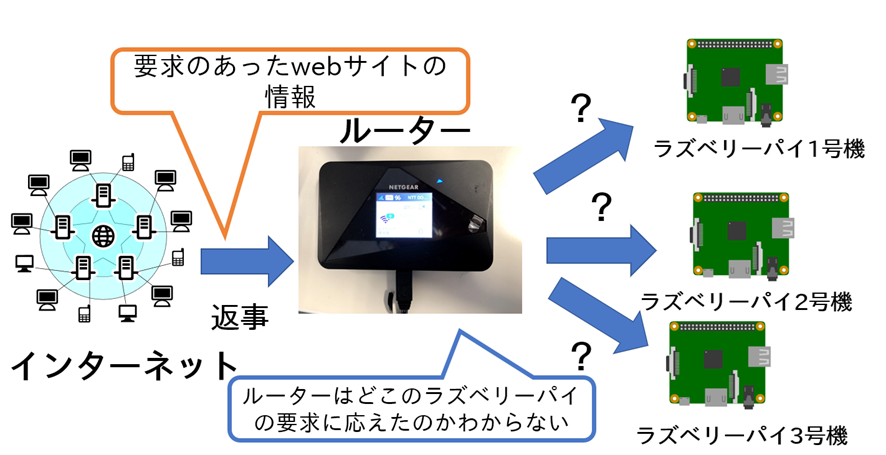
\includegraphics[width=0.85\textwidth]{../../asset/image/ome7-img015.png}
\end{center}

どれかしらのラズベリーパイからwebサイトへの要求があり、ルータを経由してインターネットに接続します。
そのあと、インターネットから要求のあったwebサイトの情報がルータにいきます。
ここで問題が発生します。
それはいったいのどのラズベリーパイの要求であったのかルータがわからないのです。
\ruby{僕}{ぼく}らが、勝手にラズベリーパイ１号機、ラズベリーパイ２号機、ラズベリーパイ３号機と名前をつけて\ruby{判断}{はんだん}していても、そのことはルータはわかりません。
そこでIPアドレスというものを使います。

ルータは自分を\ruby{含}{ふく}め、ローカルIPアドレスを割り当てています。このローカルIPアドレスでラズベリーパイを見分けています。

\begin{center}
	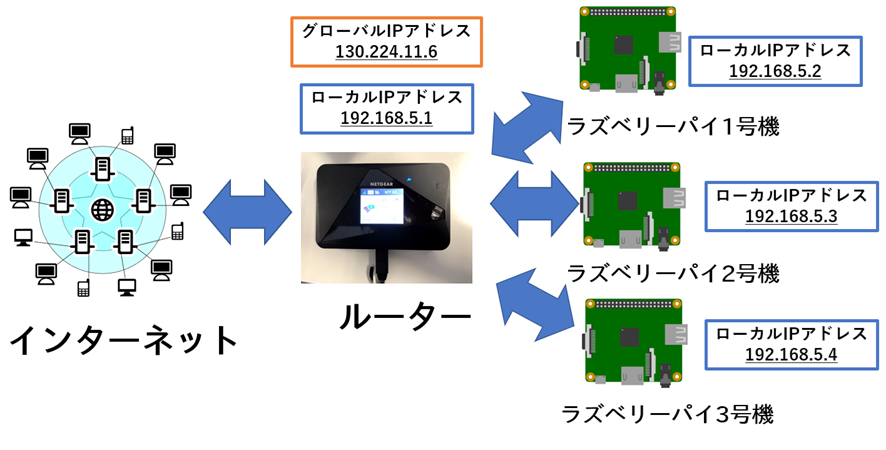
\includegraphics[width=\textwidth]{../../asset/image/ome7-img016.png}
\end{center}

\begin{tcolorbox}[title=\useOmetoi,breakable]
  \begin{enumerate}
    \addquiz{ルータはラズベリーパイたちを見分けるために何を割り当てていますか。}
  \end{enumerate}
\end{tcolorbox}

% \refstepcounter{Question}\theQuestion　ルータはラズベリーパイたちを見分けるために何を割り当てていますか。\label{P:slide_p15}\label{Q:globalIP}\\

% \refstepcounter{Exercise}

\clearpage

%
% subsection 6.2.5
%
\subsection{ポケットWi-FiルータのグローバルIPアドレスを調べよう\label{E:router}}

\begin{minipage}[b]{0.58\textwidth}
	ターミナルを開き、”curl	inet-ip.info”とコマンドを入力して、自分のラズベリーパイが接続しているWi-FiルータのグローバルIPアドレスを確認しましょう。

	curlコマンドはインターネットから情報を取ってくるときに使用します。
	今回は”inet-ip.info”というサイトからグローバルIPアドレスを調べてターミナルに\ruby{表示}{ひょうじ}させています。
	webブラウザから”inet-ip.info”にアクセスしてみると右の図のような形でグローバルIPアドレスを確認することもできます。
\end{minipage}
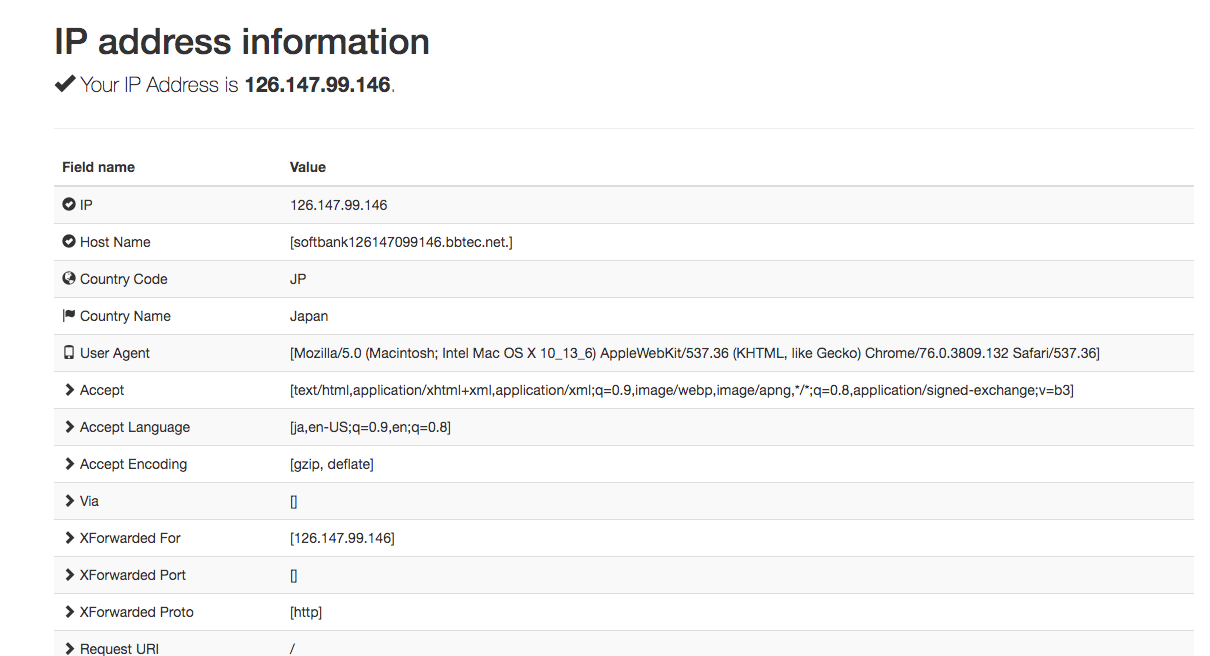
\includegraphics[width=0.4\textwidth]{../../asset/image/ome7-img017.png}

\bigskip

{\bfseries 方法}

\begin{center}
	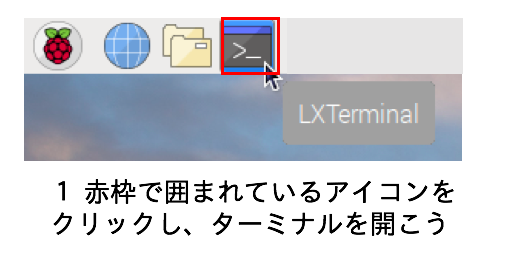
\includegraphics[width=0.85\textwidth]{../../asset/image/ome7-img007.png}
	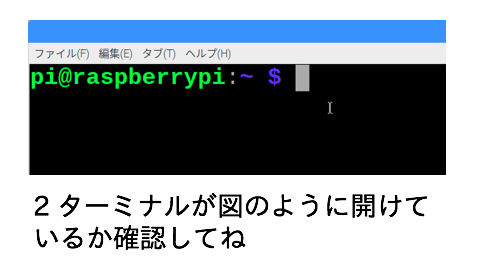
\includegraphics[width=0.85\textwidth]{../../asset/image/ome7-img008.png}
\end{center}

\clearpage

\begin{center}
	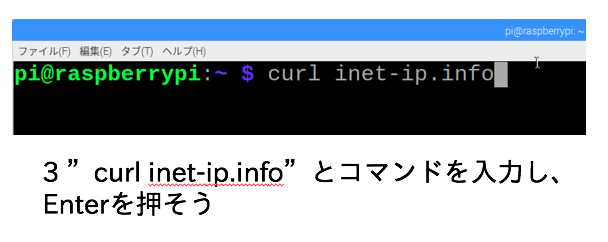
\includegraphics[width=0.85\textwidth]{../../asset/image/ome7-img018.png}
	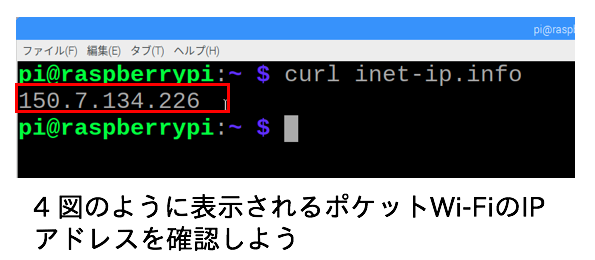
\includegraphics[width=0.85\textwidth]{../../asset/image/ome7-img019.png}
\end{center}

調べたポケットWi-FiのグローバルIPアドレスを書こう
\begin{center}
	\fbox{
		\parbox{0.8\textwidth}{
		\hspace{0pt}
		\vspace{3\baselineskip}
		}
	}
\end{center}

% \begin{table}[htbp]
% 	\centering
% 	% \caption{文字タイプ表}
% 	\begin{tabular}{|c|}
% 	\hline
% 	　　　　　　　　　　　　　　　　　　　　　　　　　　　　　　　　　　　　　　　　　　　　　　　　　　　　　　　\\
% 	　　　　　　　　　　　　　　　　　　　　　　　　　　　　　　　　　　　　　　　　　　　　　　　　　　　　　　　\\
% 	　　　　　　　　　　　　　　　　　　　　　　　　　　　　　　　　　　　　　　　　　　　　　　　　　　　　　　　\\
% 	　　　　　　　　　　　　　　　　　　　　　　　　　　　　　　　　　　　　　　　　　　　　　　　　　　　　　　　\\
% 	　　　　　　　　　　　　　　　　　　　　　　　　　　　　　　　　　　　　　　　　　　　　　　　　　　　　　　　\\

% 	\hline
% 	\end{tabular}
% \end{table}


% \flushleft

グループの友達が調べたポケットWi-FiのグローバルIPアドレスも教えてもらって書こう
\begin{center}
	\fbox{
		\parbox{0.8\textwidth}{
		\hspace{0pt}
		\vspace{3\baselineskip}
		}
	}
\end{center}

\clearpage

%
% subsection 6.2.6
%
\subsection{ポート番号とは}\label{P:port}
% \refstepcounter{PagePtr}

前のページではみんなはラズベリーパイがどのようにインターネットにつながっているのか理解してくれたと思います。
ここではさらにポート番号について\ruby{知識}{ちしき}を深めましょう。
IPアドレスは通信相手となる別のネットワークのコンピュータを特定することができます。
しかし、コンピュータでは\ruby{通常}{つうじょう}、多くのプログラム（機能）が動作していて、IPアドレスを指定するだけでは、どのプログラムと接続するかを区別できません。
そこでコンピュータ上の、\underline{どのプログラムと接続するかを指定するためにポート番号が用いられます}。
下の図は小学校を例にしています。

\begin{center}
	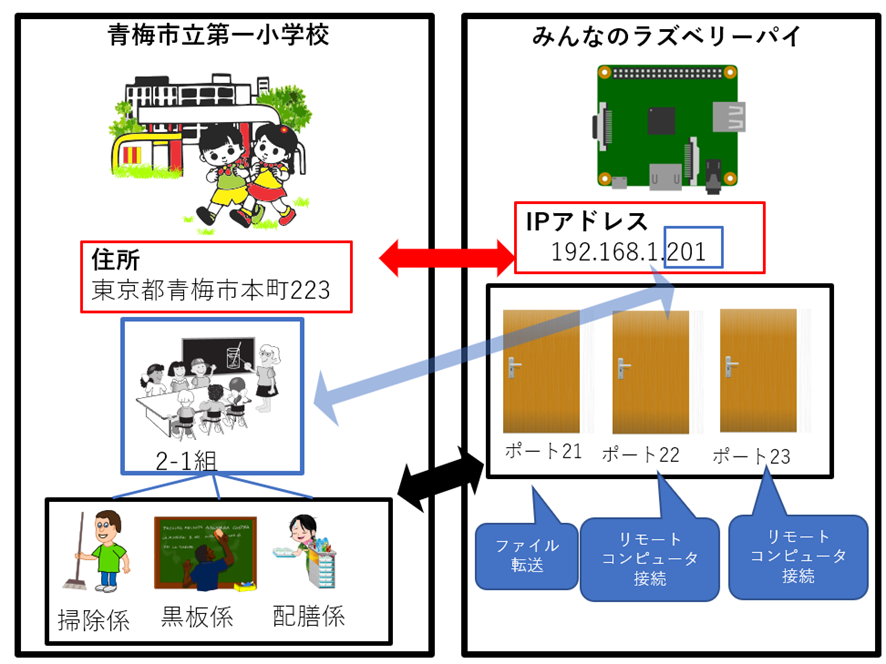
\includegraphics[width=0.85\textwidth]{../../asset/image/ome7-img020.png}
\end{center}

青梅市立第一小学校の住所がみんなのラズベリーパイのIPアドレスに\ruby{対応}{たいおう}しており、IPアドレスの\ruby{末尾}{まつび}の201（青で囲まれている）が小学校のクラスに対応しています。
皆さんの学校でも生徒にはそれぞれ係という役割が\ruby{与}{あた}えられていますね。
例えば、プリントなどの\ruby{配布物}{はいふぶつ}を配る配り係、黒板を使い終わったらきれいにする黒板係、教室の\ruby{窓}{まど}をきれいにする窓ふき係などこれらの係に相当するものがラズベリーパイにもあり、それが\underline{ポート}です。
ポート21はファイル転送用の働きをする\ruby{担当}{たんとう}で、ポート22と23は他のコンピュータに接続する担当です。
ポートには役割がありインターネットの通信はファイル転送であったり、他のコンピュータに接続して\ruby{遠隔}{えんかく}操作したり、webページにアクセスしたりといろいろあります。
なので、その分のポートを用意しておき、役割を与え、対応している役割のときに\ruby{頑張}{がんば}ってもらう仕組みになっています。
みんなのラズベリーパイやパソコン、サーバにはポートは何個あるのか調べてみるのも面白いですね。

\clearpage

\begin{tcolorbox}[title=\useOmetoi,breakable]
  \begin{enumerate}
    \addquiz{ポート番号はどのようなことに使われますか。\label{Q:portUsage}}
  \end{enumerate}
\end{tcolorbox}

ここでは実際にポートはネットワーク上ではどのように使うのか、下の図を見てみましょう。

\begin{center}
	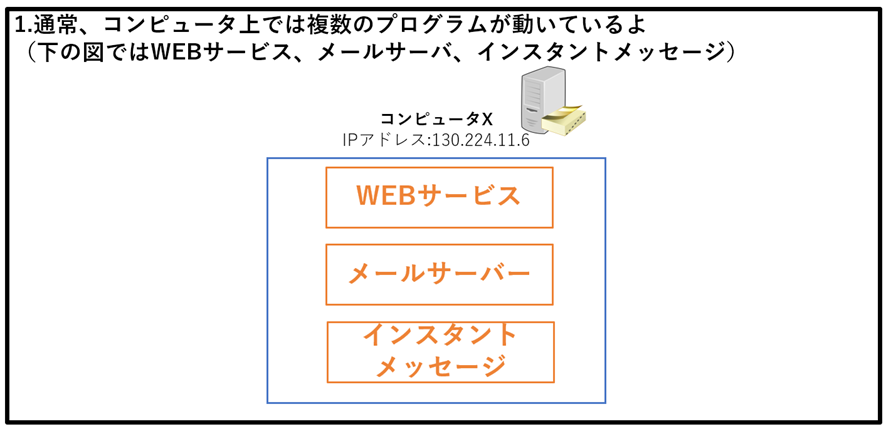
\includegraphics[width=0.97\textwidth]{../../asset/image/ome7-img021.png}
	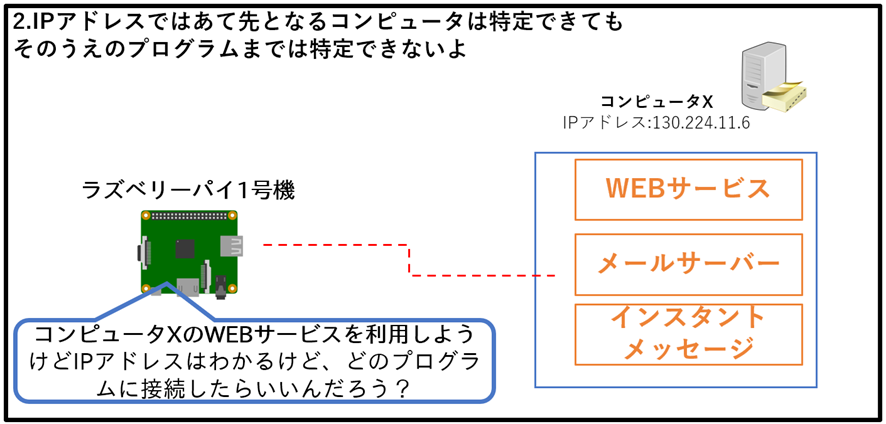
\includegraphics[width=0.97\textwidth]{../../asset/image/ome7-img022.png}
\end{center}

\clearpage

\begin{center}
	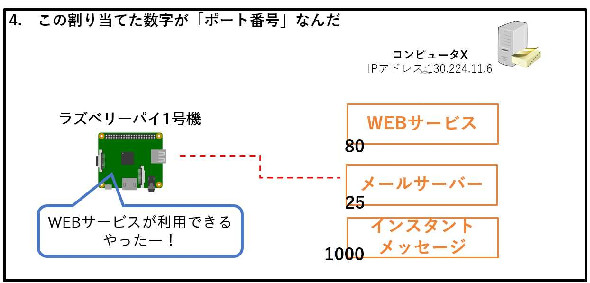
\includegraphics[width=0.97\textwidth]{../../asset/image/ome7-img024.png}
\end{center}

さらにラズベリーパイ側のポートはラズベリーパイが自動で割当ており、そこからデータを受け取っています。

\begin{center}
	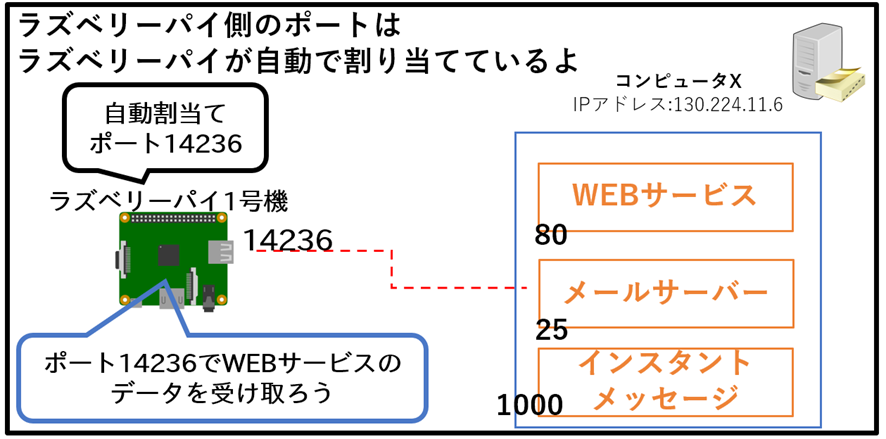
\includegraphics[width=0.97\textwidth]{../../asset/image/ome7-img025.png}\label{P:slide_p18}
\end{center}

コンピュータXのようにネット上にサービスを\ruby{提供}{ていきょう}するコンピュータを\underline{サーバ}と言います。

ラズベリーパイ１号機のようにサーバからサービスを受けるコンピュータを\underline{クライアント}言います。

これらのポートが今\ruby{現在}{げんざい}どのようなことに使われているのか\textbf{\ref{P:port}で確認してみましょう。}


\begin{tcolorbox}[title=\useOmetoi,breakable]
  \begin{enumerate}
    \addquiz{コンピュータ上のプログラム（サービス）を判断するためになにが用いられていますか。\label{Q:port}}
  \end{enumerate}
\end{tcolorbox}

\clearpage

%
% subsection 6.2.7
%
\subsection{開いているポートを調べてみよう}
% \addtocounter{Exercise}{-1}\refstepcounter{Exercise}\label{port}

ターミナルを開き、”nmap
localhost”とコマンドを入力し、ポートについて知ろう

\bigskip

{\bfseries 方法}

\begin{center}
	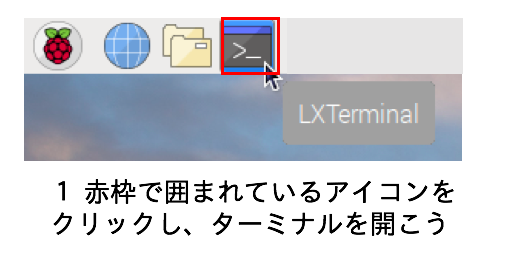
\includegraphics[width=0.85\textwidth]{../../asset/image/ome7-img007.png}
	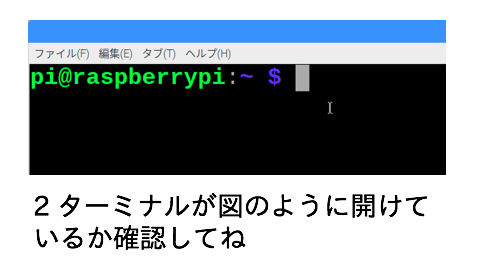
\includegraphics[width=0.85\textwidth]{../../asset/image/ome7-img008.png}
\end{center}

\clearpage

\begin{center}
	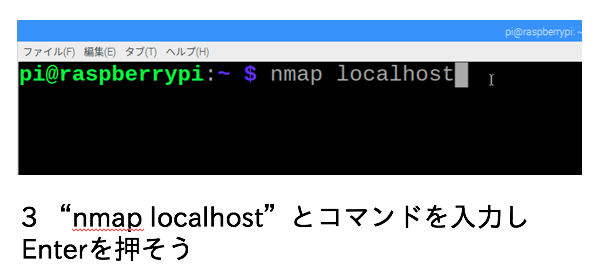
\includegraphics[width=0.85\textwidth]{../../asset/image/ome7-img032.png}
	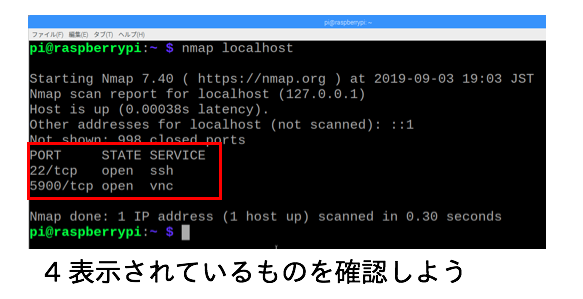
\includegraphics[width=0.85\textwidth]{../../asset/image/ome7-img031.png}
\end{center}

\bigskip

{\bfseries 自分のラズベリーパイに表示されたものを下の表に書こう}

\begin{table}[htbp]
	\centering
	% \caption{文字タイプ表}
	\begin{tabular}{|c|c|c|}
	\hline
		PORT　　　　　　　　　　　& STATE　　　　　　　　　　& SERVICE　　　　　　　　　　\\
		\hline
		& & \\
		\hline
		& & \\
		\hline
		& & \\
		\hline
		& & \\
		\hline
	\end{tabular}
  \end{table}



% {\bfseries
serviceに出てきた言葉をインターネットを使って調べよう。
皆さんにとっては\ruby{難}{むず}しい言葉が多いと思います。
それでも自分で調べてみましょう。
それが知識を深める近道です。\\
ポートが開いていない場合、コマンドは何も表示せず、
改行が起こるだけのこともあります。
% }

\clearpage

%
% subsection 6.2.8
%
\subsection{コラム DNS（Domain Name System）について}
\refstepcounter{PagePtr}\label{P:DNS}

IPアドレスは住所であり、それがわからないとサーバのサービスをうけることはできません。
ですが以下の図のようなことが起こることがあります。

\begin{center}
	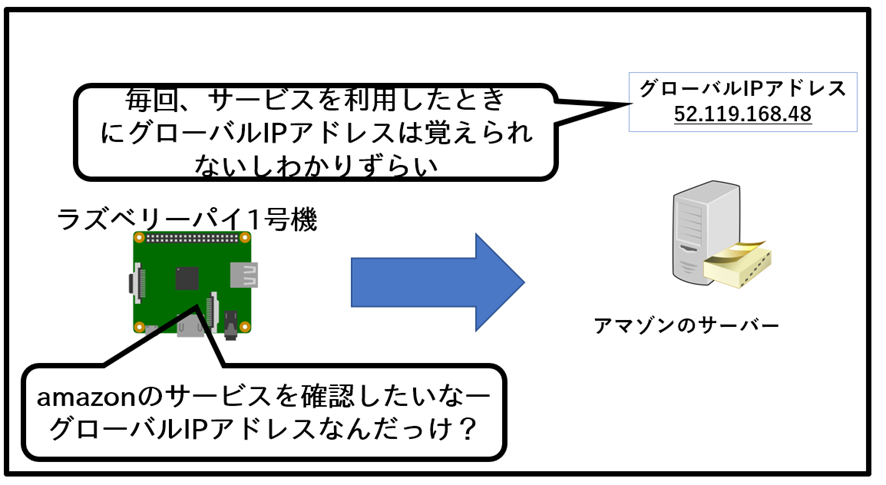
\includegraphics[width=0.97\textwidth]{../../asset/image/ome7-img026.png}
\end{center}

そこで、DNSサーバと言うものを作り、一度そこに”amazon.co.jp”のグローバルIPアドレスを教えてもらってサーバに接続しています。

\begin{center}
	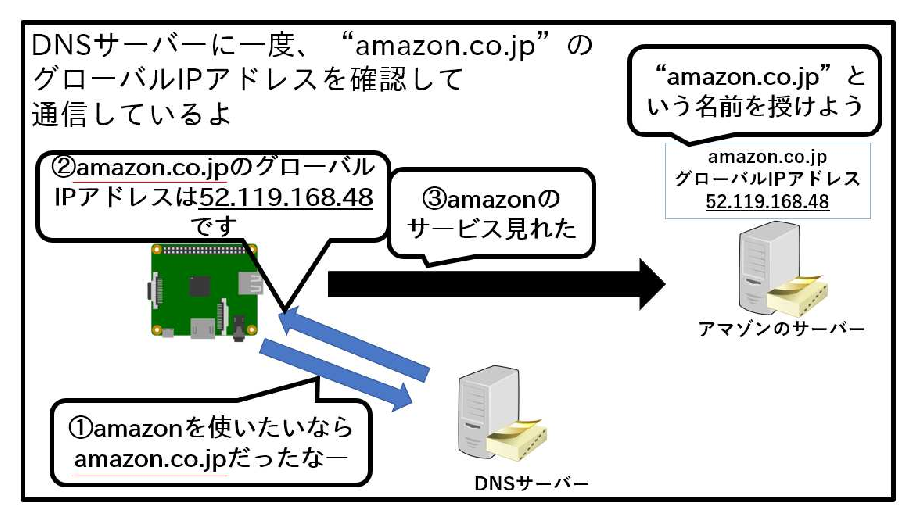
\includegraphics[width=0.97\textwidth]{../../asset/image/ome7-img027}
\end{center}


\clearpage

\begin{center}
	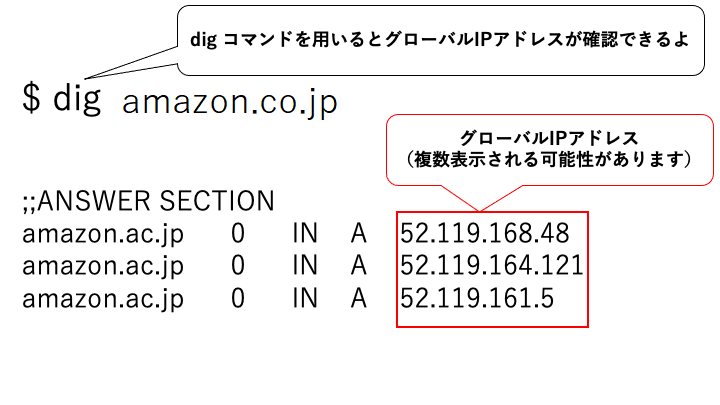
\includegraphics[width=0.8\textwidth]{../../asset/image/ome7-img028_1.png}
\end{center}

\begin{tcolorbox}[title=\useOmetoi,breakable]
  \begin{enumerate}
    \addex{ターミナルを開き、”dig	amazon.co.jp”を実行してグローバルIPアドレスを確認しよう。\label{Q:dig}}
  \end{enumerate}
\end{tcolorbox}

\clearpage

%
% subsection 6.2.9
%
\subsection{NATについて}

教科書の前のページでローカルIPアドレスとグローバルIPアドレスが存在することを皆さんは知りました。ここではもっと細かくIPアドレスを用いたインターネット接続を勉強しましょう。
インターネットに接続するコンピュータは自分自身を示すIPアドレスとして世界で\ruby{唯一}{ゆいつ}のグローバルIPアドレスを使わなければならないのです。
みなさんのラズベリーパイにはローカルIPアドレスしか割り当てられていませんので、このままではインターネットをすることはできません。
そこでNAT（Network Address Translation）というものを用います。
このNATはルータが行っていて、送信元のローカルIPアドレスをグローバルIPアドレスに変換して通信を行っています。
具体的にはどのようになっているのか下の図をみて確認してみましょう。


\begin{center}
	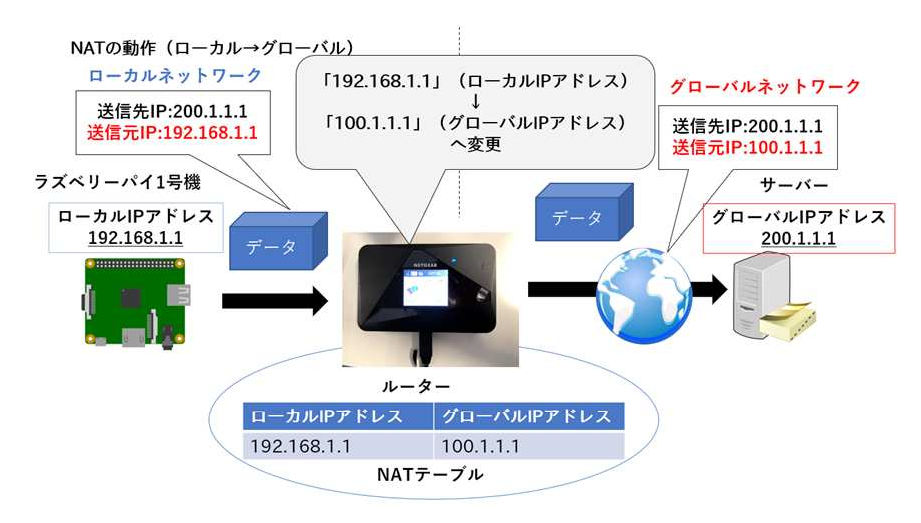
\includegraphics[width=0.8\textwidth]{../../asset/image/ome7-img029}
\end{center}

\clearpage

ラズベリーパイ1号機からサーバにデータの送信先IPアドレスは200.1.1.1（グローバルIPアドレス）、送信元IPアドレスは192.168.1.1（ローカルIPアドレス）です。
NATを行うルータは、プライベートアドレスとグローバルアドレスの\ruby{境界}{きょうかい}に位置しています。
ここでルータは、ラズベリーパイから送信されたデータの送信元IPアドレス192.168.1.1を、グローバルIPアドレスの「100.1.1.1」に変換して転送します。このときルータは、その変換情報をNATテーブルに記録しています。この記録が、「返ってくるデータ」、つまりサーバからラズベリーパイへ送られるデータの転送時に役立ちます。次の図を見てください。


\begin{center}
	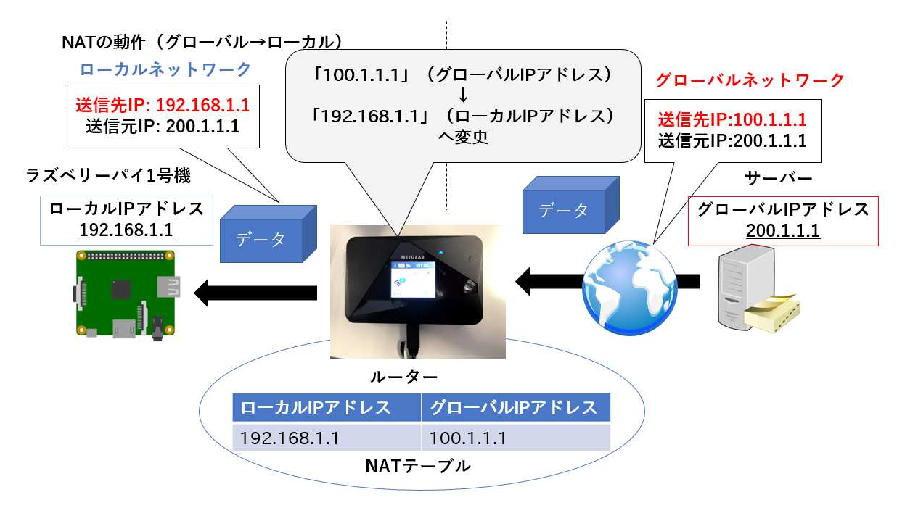
\includegraphics[width=0.8\textwidth]{../../asset/image/ome7-img030}
\end{center}

サーバからラズベリーパイへの返事のデータの送信先IPアドレスは「100.1.1.1」、送信元IPアドレス「200.1.1.1」になりますね。
データがルータへ転送されてくると、ルータはNATテーブルを確認して、送信元IPアドレスを「100.1.1.1」から元の「192.168.1.1」へ変換します。
これにより返りのデータの通信が可能になるのです。NATによって送信元のローカルIPアドレスをグローバルIPアドレスに変換して通信をおこなっているおかげでみんなはインターネットを利用できています。

\clearpage\end{document}
